\documentclass[12pt,letterpaper]{article}
\usepackage{graphicx,textcomp}
\usepackage{natbib}
\usepackage{setspace}
\usepackage{fullpage}
\usepackage{color}
\usepackage[reqno]{amsmath}
\usepackage{amsthm}
\usepackage{fancyvrb}
\usepackage{amssymb,enumerate}
\usepackage[all]{xy}
\usepackage{endnotes}
\usepackage{lscape}
\newtheorem{com}{Comment}
\usepackage{float}
\usepackage{hyperref}
\newtheorem{lem} {Lemma}
\newtheorem{prop}{Proposition}
\newtheorem{thm}{Theorem}
\newtheorem{defn}{Definition}
\newtheorem{cor}{Corollary}
\newtheorem{obs}{Observation}
\usepackage[compact]{titlesec}
\usepackage{dcolumn}
\usepackage{tikz}
\usetikzlibrary{arrows}
\usepackage{multirow}
\usepackage{xcolor}
\newcolumntype{.}{D{.}{.}{-1}}
\newcolumntype{d}[1]{D{.}{.}{#1}}
\definecolor{light-gray}{gray}{0.65}
\usepackage{url}
\usepackage{listings}
\usepackage{color}

\definecolor{codegreen}{rgb}{0,0.6,0}
\definecolor{codegray}{rgb}{0.5,0.5,0.5}
\definecolor{codepurple}{rgb}{0.58,0,0.82}
\definecolor{backcolour}{rgb}{0.95,0.95,0.92}

\lstdefinestyle{mystyle}{
	backgroundcolor=\color{backcolour},   
	commentstyle=\color{codegreen},
	keywordstyle=\color{magenta},
	numberstyle=\tiny\color{codegray},
	stringstyle=\color{codepurple},
	basicstyle=\footnotesize,
	breakatwhitespace=false,         
	breaklines=true,                 
	captionpos=b,                    
	keepspaces=true,                 
	numbers=left,                    
	numbersep=5pt,                  
	showspaces=false,                
	showstringspaces=false,
	showtabs=false,                  
	tabsize=2
}
\lstset{style=mystyle}
\newcommand{\Sref}[1]{Section~\ref{#1}}
\newtheorem{hyp}{Hypothesis}

\begin{document} 
	
\title{Problem Set 2}
\author{Applied Statistical Analysis 1}
\date{Maiia Skrypnyk 23371609}

	\maketitle
	\section*{Instructions}
\begin{itemize}
	\item Please show your work! You may lose points by simply writing in the answer. If the problem requires you to execute commands in \texttt{R}, please include the code you used to get your answers. Please also include the \texttt{.R} file that contains your code. If you are not sure if work needs to be shown for a particular problem, please ask.
	\item Your homework should be submitted electronically on GitHub.
	\item This problem set is due before 23:59 on Sunday October 15, 2023. No late assignments will be accepted.

\end{itemize}

	
	\vspace{.5cm}
	\section*{Question 1: Political Science}
		\vspace{.25cm}
	The following table was created using the data from a study run in a major Latin American city.\footnote{Fried, Lagunes, and Venkataramani (2010). ``Corruption and Inequality at the Crossroad: A Multimethod Study of Bribery and Discrimination in Latin America. \textit{Latin American Research Review}. 45 (1): 76-97.} As part of the experimental treatment in the study, one employee of the research team was chosen to make illegal left turns across traffic to draw the attention of the police officers on shift. Two employee drivers were upper class, two were lower class drivers, and the identity of the driver was randomly assigned per encounter. The researchers were interested in whether officers were more or less likely to solicit a bribe from drivers depending on their class (officers use phrases like, ``We can solve this the easy way'' to draw a bribe). The table below shows the resulting data.

\newpage
\begin{table}[h!]
	\centering
	\begin{tabular}{l | c c c }
		& Not Stopped & Bribe requested & Stopped/given warning \\
		\\[-1.8ex] 
		\hline \\[-1.8ex]
		Upper class & 14 & 6 & 7 \\
		Lower class & 7 & 7 & 1 \\
		\hline
	\end{tabular}
\end{table}

\begin{enumerate}
Let's create a contingency table (as a matrix) with the given data:
		\lstinputlisting[language=R, firstline=4, lastline=10]{PS02MS.R} 
		 
 \textbf{(a)
		Calculate the $\chi^2$ test statistic by hand/manually (even better if you can do "by hand" in \texttt{R}).\\} 

\textit{\textit{Fe=(row total/grand total) * column total}}
	\lstinputlisting[language=R, firstline=14, lastline=47]{PS02MS.R}  
	
		\begin{figure}[h!]
		\centering
		\label{fig:chisquared}
		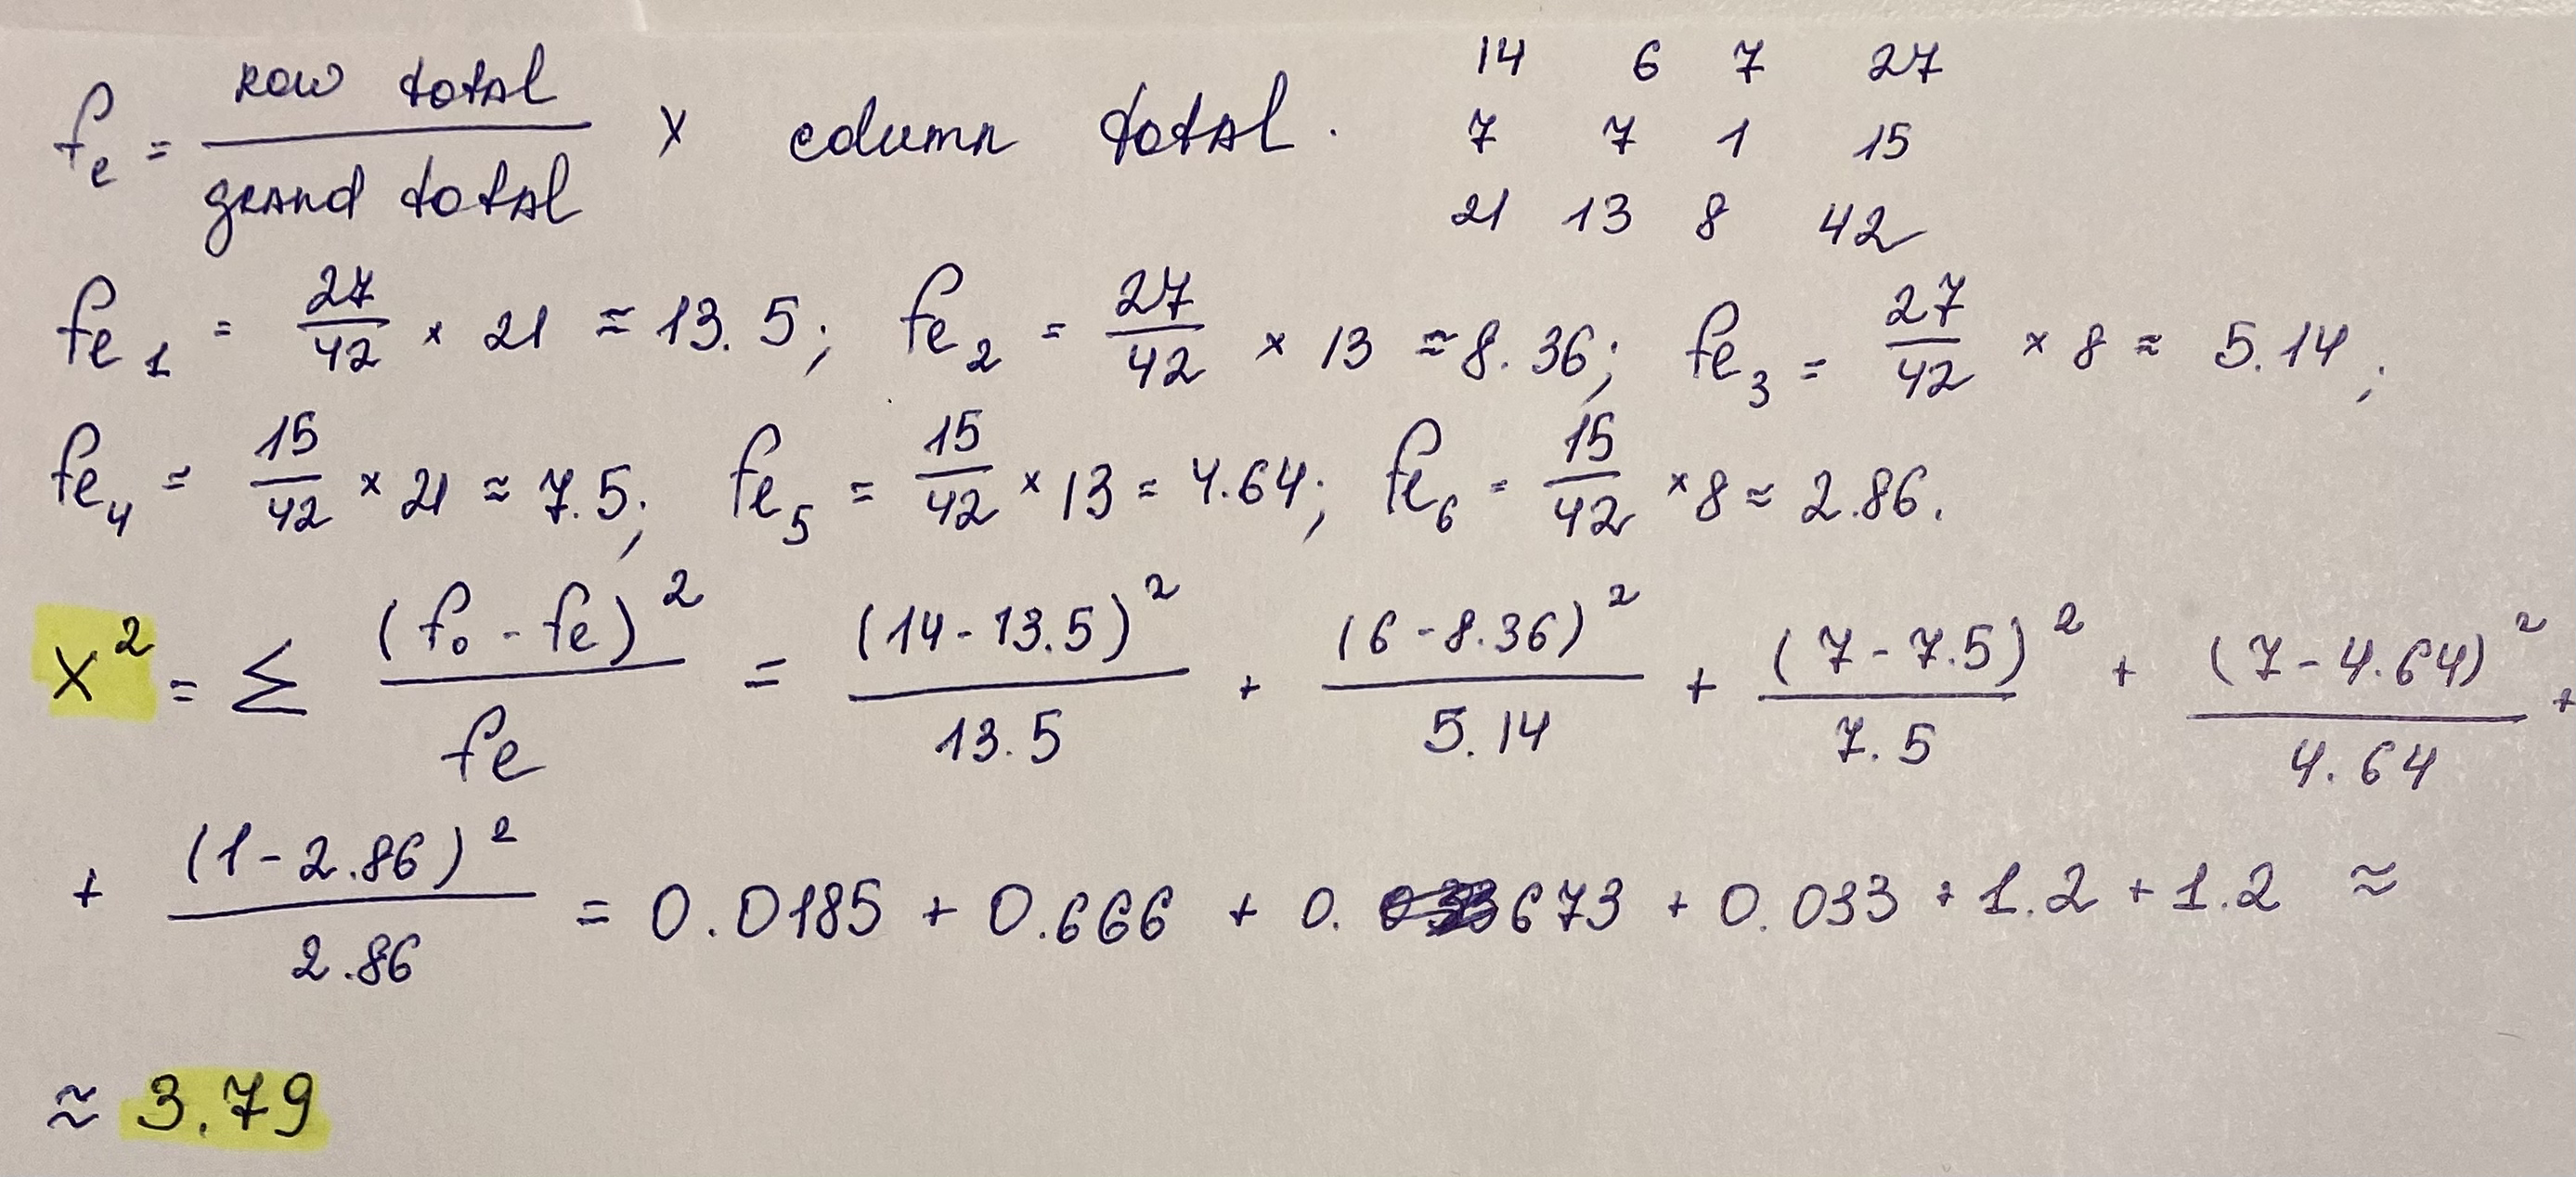
\includegraphics[width=0.9\textwidth]{chisquared.png}
	\end{figure}		
	
My result by hand was 3.79, R-calculations also gave us 3.79. 
That's great, but let's also check via an embedded formula:
\lstinputlisting[language=R, firstline=51, lastline=53]{PS02MS.R}  
	\textbf{(b)
	Now calculate the p-value from the test statistic you just created (in \texttt{R}).\footnote{Remember frequency should be $>$ 5 for all cells, but let's calculate the p-value here anyway.}  What do you conclude if $\alpha = 0.1$?\\}
	
		\lstinputlisting[language=R, firstline=56, lastline=57]{PS02MS.R}  

If alpha = 0.1, our p-value (0.15) is larger than 0.1, therefore we FAIL TO REJECT that the variables Class and Police Response (solicitation of bribery) are statistically independent (H0).

 \textbf{(c) Calculate the standardized residuals for each cell and put them in the table below.}
\vspace{0.2cm}

If we extract the 'residuals' from our R-run Chi-squared test, 
we will get the results that are Standardized residuals/Pearson's residuals \href{https://scholarworks.umass.edu/cgi/viewcontent.cgi?article=1269&context=pare#:~:text=There%20are%20at%20least%20four,the%20chi%2Dsquare%20test%20result}{(p.3 here)}: 

\textit{(F observed - F expected) / square root of F expected}
		\lstinputlisting[language=R, firstline=67, lastline=67]{PS02MS.R}  
	
	\begin{figure}[h!]
		\centering
		\label{fig:residuals}
		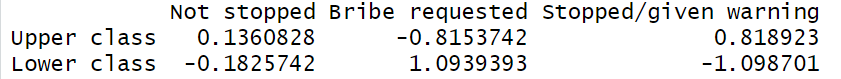
\includegraphics[width=0.9\textwidth]{residuals.png}
	\end{figure}
	
		\begin{figure}[h!]
		\centering
		\label{fig:myresiduals}
		\includegraphics[width=0.9\textwidth]{myresiduals.png}
	\end{figure}				
	
I calculated them by hand and have the same numbers, BUT! 
They are not what we are looking for.

From my understanding, we are looking for what Agresti and Finlay call standardized residuals as well, but they are also called \textbf {Adjusted Standardized Residuals (ASR)}: \textit {(F observed - F expected) / square root of (F expected * (1-row proportion) * (1-column proportion)}


We can also extract them from our Chi-squared test results, but they are stored under 'stdres':
	\lstinputlisting[language=R, firstline=80, lastline=80]{PS02MS.R}  
	
		\begin{figure}[h!]
		\centering
		\label{fig:stdres}
		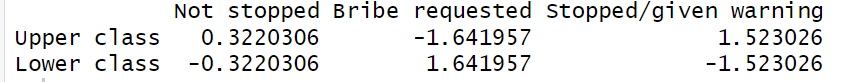
\includegraphics[width=0.9\textwidth]{stdres.png}
	\end{figure}		
\begin{flushleft}
	And now let's calculate them manually in R:
\end{flushleft}

		\lstinputlisting[language=R, firstline=84, lastline=95]{PS02MS.R}  
		
\begin{figure}[h!]
	\centering
	\label{fig:mystdres}
	\includegraphics[width=0.7\textwidth]{mystdres.png}
\end{figure}	
	\vspace{1cm}
	
\begin{flushleft}
	\centering
	\textit{(By-hand calculations support the R-calculated results)} 
\end{flushleft}
		\vspace{3cm}
	
\begin{flushleft}Filling our table with the ASRs: \end{flushleft}
	\begin{table}[h]
		\centering
		\begin{tabular}{l | c c c }
			& Not Stopped & Bribe requested & Stopped/given warning \\
			\\[-1.8ex] 
			\hline \\[-1.8ex]
			Upper class  & 0.322 & -1.64 & 1.52  \\
			\\
			Lower class & -0.322 &  1.64  & -1.52   \\
			
		\end{tabular}
	\end{table}
	
\textbf{(d) How might the standardized residuals help you interpret the results?}  

\textit{(Agresti \& Finlay, 2009, p. 230)}. A residual is the difference between an observed and expected cell frequency. Positive residual = in this cell, the observed frequency exceeds the value that independence predicts; negative residual = the observed frequency is smaller than independence predicts. A denominator in ASR is the standard error (uses the marginal proportions for the row and the column in which the cell falls), presuming H0 is true. When H0: independence is true, the ASRs have a large-sample standard normal distribution (mean 0, sd 1). 

A large ASR provides evidence against independence in the cell. When H0 is true, there is only about 5\% that any particular ASR exceeds 2 in absolute value. Values below -3 or above +3 are very convincing evidence of a true effect in that cell.

In our case, none of the residuals exceeds 2, which adds to our conclusion of failing to reject H0. 

Also, given the same column, if the observed value is larger than the expected value in one cell, the reverse must happen in the other cell -- the differences have the same magnitude but different sign in the two cells, implying the same pattern for their ASRs.

\begin{itemize}
	\item \textbf {'Not stopped' column:} \\
	\underline{Upper class:} \textit{the observed value is above the expected.} This means that the observed number of cases of the police not stopping the upper-class drivers for their misdeeds (illegal left turn) is higher that it was expected under H0:independence. We expected to see fewer cases where the upper-class drivers were not stopped. In reality, they were not stopped more frequently.\\
	
	\underline{Lower class:} \textit {the observed value is below the expected}. Correspondingly, we expected to see more cases of the lower class drivers not being stopped by the police. In reality, they were not stopped less frequently.\\
	
	For the next two columns, we can observe that ASRs are even greater in value than in the first column, which means they are more further away from what would have been expected under H0:independence. 
	
	\item \textbf {'Bribe requested' column:}\\
	\underline{Upper class: }\textit{the observed value is below the expected.} We expected to see more bribes being requested from the upper class drivers, but in reality they turned up being requested a bribe in fewer cases than we anticipated.\\
	
	\underline{Lower class:} \textit {the observed value is above the expected}. Correspondingly, the lower class drivers were expected to be requested a bribe less often than they really were.\\
	\item \textbf {'Stopped/given warning' column:}\\
	\underline{Upper class:} \textit{the observed value is above the expected.} It was expected that the upper class drivers would be less frequently stopped/given warning by the police. In reality, they were stopped/given warning more often.\\
	
	\underline{Lower class:} \textit {the observed value is below the expected}. Correspondingly, we expected to see the lower class drivers being stopped more by the police than they really were.
	\vspace{1cm}
	
\textbf{TO SUM UP}, the interpretation of the above-given residuals brings us to a following conclusion:
\item  Bribe solicitation is likely to be influenced by the class (establishing causality not association because this is a controlled experiment (\href{https://www.scribbr.com/frequently-asked-questions/correlational-vs-experimental-research/}{source}).
\item In this case, the police is more likely to \underline{not} stop the upper class drivers as compared to the lower class drivers, and also \underline{not} to request a bribe from the former. Therefore, the lower class drivers are expected to be more targeted by the police in these cases. Though, it is interesting to note that the upper class drivers are still not 'exempt' of any interaction with the police, because they are stopped or given warning in more number of cases than we were expecting under H0:independence.

\end{itemize}


\end{enumerate}
\newpage

\section*{Question 2: Economics}
Chattopadhyay and Duflo were interested in whether women promote different policies than men.\footnote{Chattopadhyay and Duflo. (2004). ``Women as Policy Makers: Evidence from a Randomized Policy Experiment in India. \textit{Econometrica}. 72 (5), 1409-1443.} Answering this question with observational data is pretty difficult due to potential confounding problems (e.g. the districts that choose female politicians are likely to systematically differ in other aspects too). Hence, they exploit a randomized policy experiment in India, where since the mid-1990s, $\frac{1}{3}$ of village council heads have been randomly reserved for women. A subset of the data from West Bengal can be found at the following link: \url{https://raw.githubusercontent.com/kosukeimai/qss/master/PREDICTION/women.csv}\\

\noindent Each observation in the data set represents a village and there are two villages associated with one GP (i.e. a level of government is called "GP"). Figure~\ref{fig:women_desc} below shows the names and descriptions of the variables in the dataset. The authors hypothesize that female politicians are more likely to support policies female voters want. Researchers found that more women complain about the quality of drinking water than men. You need to estimate the effect of the reservation policy on the number of new or repaired drinking water facilities in the villages.
\vspace{.5cm}
\begin{figure}[h!]
	\caption{\footnotesize{Names and description of variables from Chattopadhyay and Duflo (2004).}}
	\vspace{.5cm}
	\centering
	\label{fig:women_desc}
	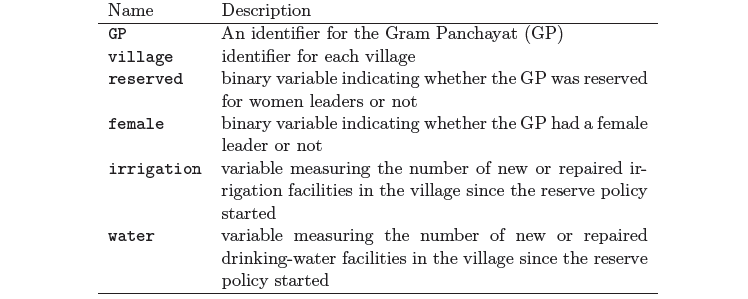
\includegraphics[width=1.1\textwidth]{women_desc_Skrypnyk.png}
\end{figure}		

\lstinputlisting[language=R, firstline=112, lastline=112]{PS02MS.R}  

\newpage
\begin{enumerate}

	\lstinputlisting[language=R, firstline=136, lastline=136]{PS02MS.R}  


\textbf{(a) State a null and alternative (two-tailed) hypothesis}. 

\noindent \begin{center}
	$y = \alpha + \beta x$\\ 
\end{center}

\begin{flushleft}
\textit{x} \textit{(input/explanatory variable)} =  reservation policy 
		(a binary variable with values, assumably, 'reserved for women' and 'not reserved for women' assigned to numerical values 0 and 1) \\
\textit{y} \textit{(output/response variable)} = number or new or repaired drinking water facilities 

\end{flushleft}


		 \textit {\textbf  {Null hypothesis:}} There reservation policy has no effect on the number of new or repaired drinking water facilities in the villages.
		 
			\textbf {\textit {Alternative hypothesis:}} There reservation policy has some effect on  the number of new or repaired drinking water facilities in the villages.} \\
		
\textbf{(b) Run a bivariate regression to test this hypothesis in \texttt{R} (include your code!).}

I will use the lm() function first (R won't lie to us re: calculations!), my by-hand calculation will be posted below.

		
	\lstinputlisting[language=R, firstline=118, lastline=119]{PS02MS.R}  
	
\begin{figure}[h!]
	\centering
	\label{fig:model}
	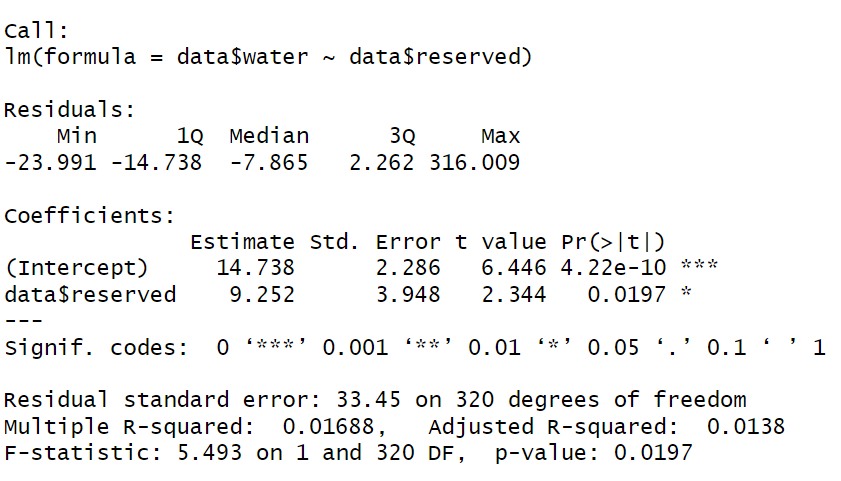
\includegraphics[width=0.7\textwidth]{model.png}
\end{figure}	
\vspace{1cm}

Now, I will calculate the bivariate regression 'by hand' (being guided by pp. 58-60 in Week 3 slides):
	\lstinputlisting[language=R, firstline=124, lastline=135]{PS02MS.R}  
	
Our slope = 9.252423.
Our intercept  = 14.73832.
\textit{(Exactly like R calculated for us with lm() function).}
	
\textbf{(c) Interpret the coefficient estimate for reservation policy.}
\end{enumerate}


\begin{center}
	$\alpha = 14.738 \\
	\begin{center}
		\beta = 9.252
	\end{center}
\end{center}
\begin{center}
	\textit{p-value} = 0.0197
\end{center}
	
\begin{itemize}
	\item As our input variable (reservation policy) is a binary variable, we can draw a conclusion that the change from no reservation policy for GP to having a reservation policy for GP is, on average, associated with a 9.252 increase in the number of new or repaired drinking water facilities. 
	\item Our p-value = 0.0197 (smaller than 0.05 threshold), so we have significant evidence to \textbf{REJECT} the null hypothesis and support the alternative hypothesis: the presence of the reservation policy has such an effect* (*once again, as this is a randomized experiment) on the number of new or repaired drinking water facilities in the village that, on average, it causes an increase of 9.252 additional water facilities in the locality.
	
\end{itemize}
	
\end{document}
